\section{Performance}
\label{sec:result}
We have tested our approaches under various parameters, based on a corpus provided by teacher Xu.
For detailed description of the corpus, please see former report.

All the tests in this section have been conducted serval times
(depending on computation cost, vary from 10 to 30)
with random selected training and testing speakers.
The average over these tests are considered as confidential result.

\subsection{Efficiency Test of our GMM}
We have extensively examined the efficiency of our implementation of GMM
compared to scikit-learn version. Test is conducted using real MFCC data with
13 dimensions, 20ms frame length. We consider the scenario when training a UBM with 256 mixtures.
We examine the time used for ten iteration.  For comparable results, we diabled
the K-means initialization process of both scikit-learn GMM implementation and
ours. Time used for ten iterations under different data size and concurrency
is recorded.

\begin{figure}[!ht]
	\begin{minipage}{0.48\linewidth}
		\centering
		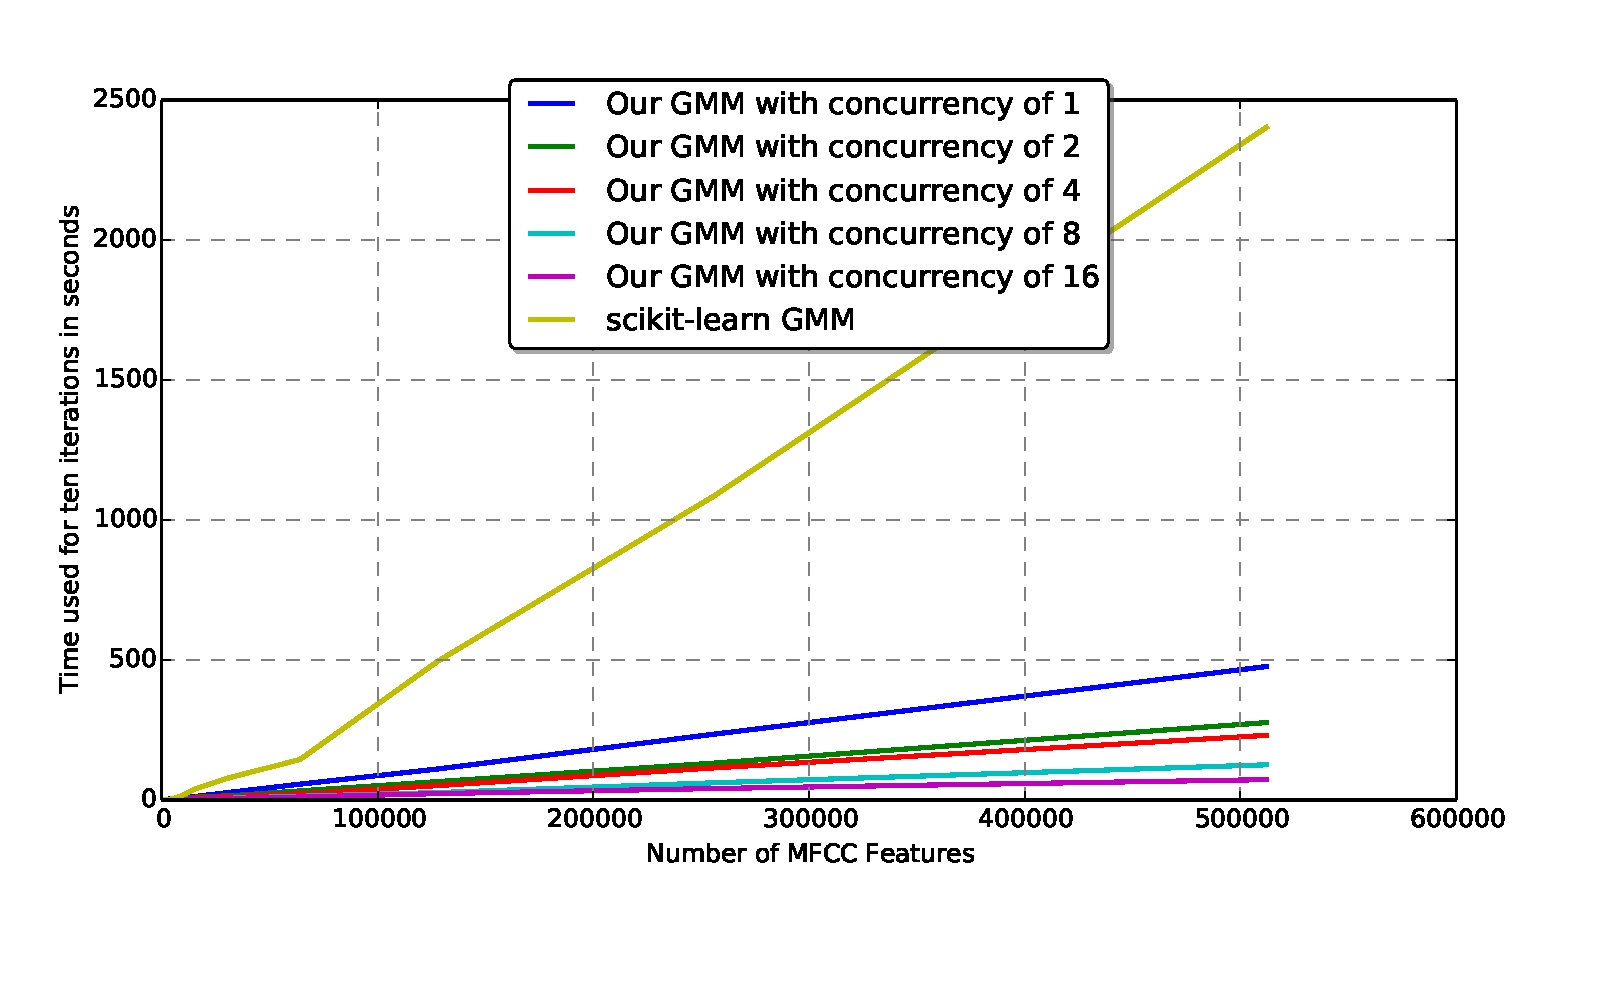
\includegraphics[width=\linewidth]{img/time-comp.pdf}
		\caption{Comparison on efficiency\label{fig:gmm_efficiency}}
	\end{minipage}
	\hfill
	\begin{minipage}{0.48\linewidth}
		\centering
		\includegraphics[width=\linewidth]{img/time-comp-small.pdf}
		\caption{Comparison on efficiency when number of MFCC features is small\label{fig:gmm_efficiency_small}}
	\end{minipage}
\end{figure}

From \figref{gmm_efficiency}, we can immediately infer that our method
is much-much more efficient than the widely used version of GMM provided
by scikit-learn when the data size grows sufficiently large.

We shall analyze in two aspect:
\begin{itemize}
    \item No concurrency

             When the number of MFCC features grows sufficiently large, our method
                shows great improvement. When training 512,000 features, our method
                is 5 times faster than comparing method.
    \item With concurrency \\
        Our method shows considerable concurrency scalability that the running time
        is approximately lineary to the number of cores using.

        When using 8-cores, our method is \textbf{$19$ times} faster than comparing
        method.
\end{itemize}


\subsection{Change in MFCC Parameters}
The following tests reveal the effect of MFCC parameters on the final accuracy.
The tests were all performed on ``Style-Reading'' corpus with 40 speakers, each with 20 seconds for enrollment
and 5 seconds for recognition.
\begin{enumerate}
  \item Different Number of Cepstrums
    \begin{figure}[H]
      \centering
      \includegraphics[width=0.7\textwidth]{img/mfcc-nceps.pdf}
    \end{figure}

  \item Different Number of Filterbanks
    \begin{figure}[H]
      \centering
      \includegraphics[width=0.7\textwidth]{img/mfcc-nfilter.pdf}
    \end{figure}

  \item Different Size of Frame
    \begin{figure}[H]
      \centering
      \includegraphics[width=0.7\textwidth]{img/mfcc-frame-len.pdf}
    \end{figure}
\end{enumerate}

\subsection{Change in LPC Parameters}
The following tests display the effect of LPC parameters on the final accuracy.
The tests were performed on ``Style-Reading'' with 40 speakers, each with 20 seconds for enrollment
and 5 seconds for recognition.
\begin{enumerate}
  \item Different Number of Coefficient
    \begin{figure}[H]
      \centering
      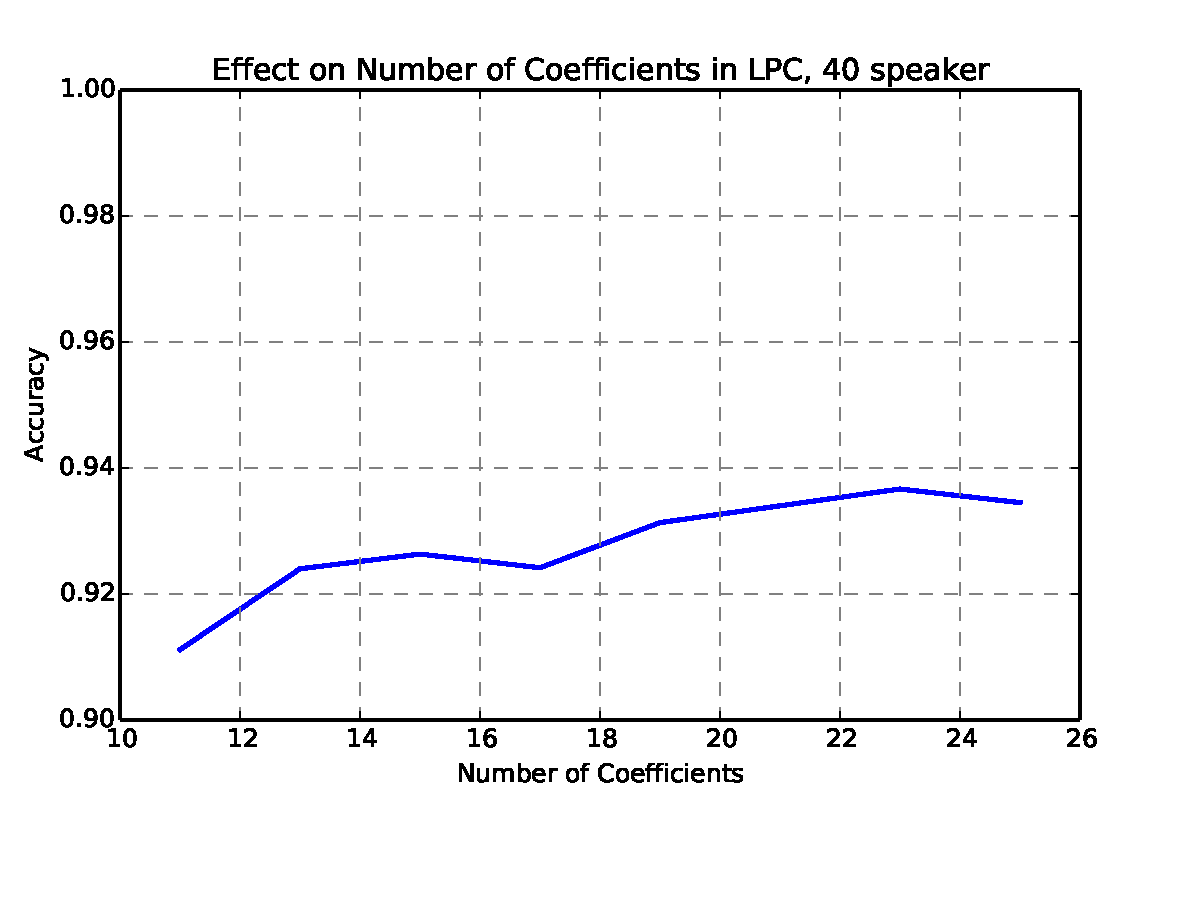
\includegraphics[width=0.7\textwidth]{img/lpc-nceps.pdf}
    \end{figure}

  \item Different Size of Frame
    \begin{figure}[H]
      \centering
      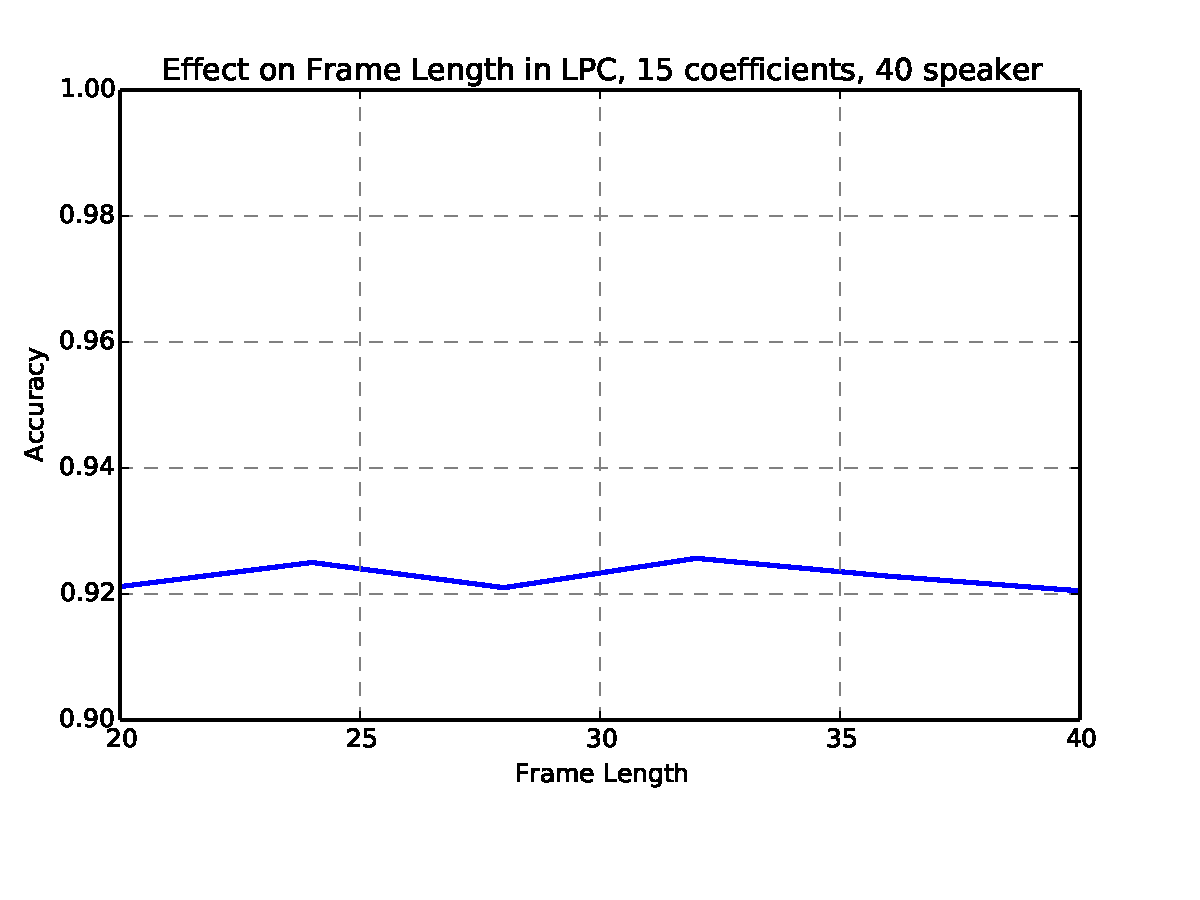
\includegraphics[width=0.7\textwidth]{img/lpc-frame-len.pdf}
    \end{figure}
\end{enumerate}

\subsection{Change in GMM Components}

We experimented on the effect of GMM Components. We found that the number of components
have slight effect on the accuracy, but a GMM with higher order might take
significantly longer time to train. Therefore we still use GMM with 32 components in our system.

\begin{figure}[H]
  \centering
  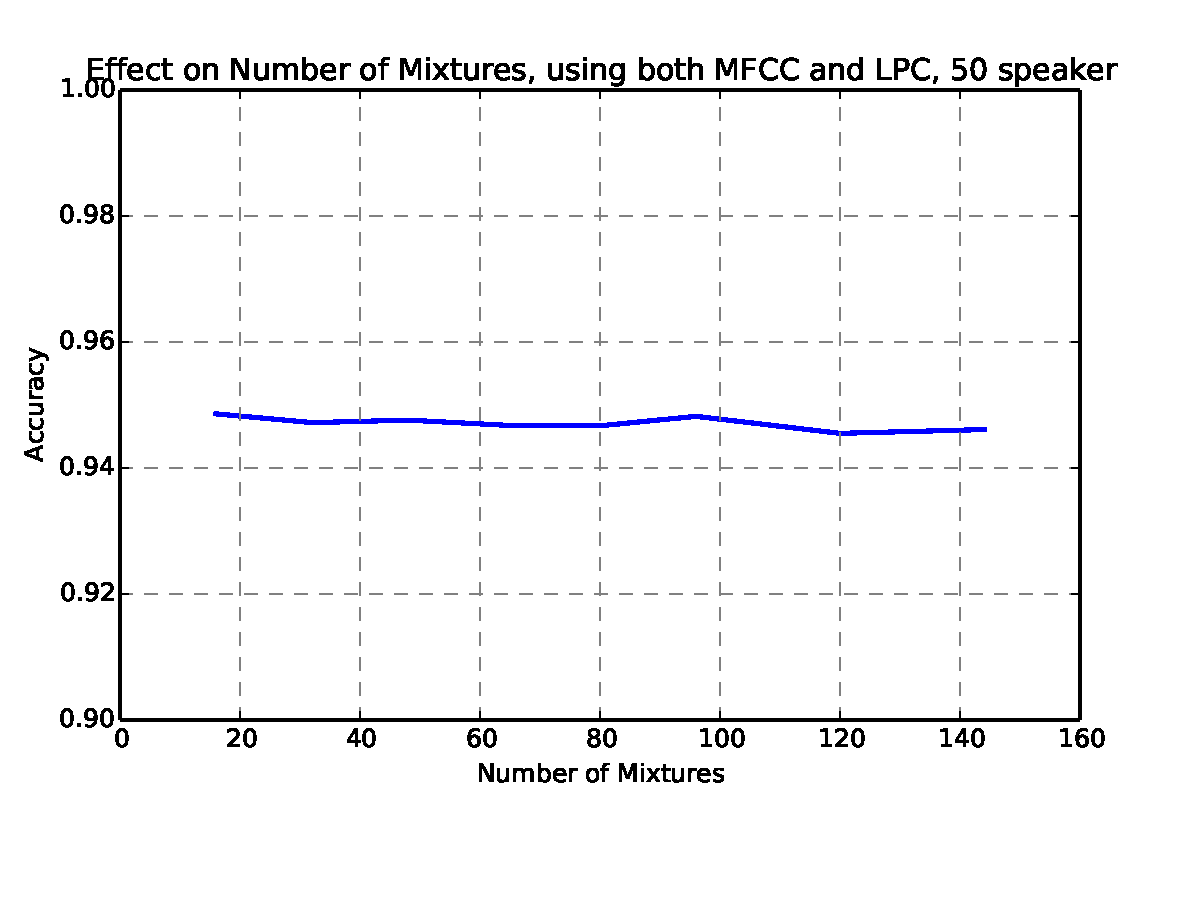
\includegraphics[width=0.7\textwidth]{img/nmixture.pdf}
\end{figure}

\subsection{Different GMM Algorithms}
We compare our implementation of GMM to GMM in scikits-learn.

The configurations of the test is as followed:
\begin{itemize}
    \item Only MFCC: frame size is $20 ms $, 19 cepstrums, 40 filterbanks
	\item Number of mixtures is set to 32, the optimal number we found previously
	\item GMM from scikit-learn, compared to our GMM.
	\item 30s training utterance and 5s test utterance
	\item 100 sampled test utterance for each user
\end{itemize}

\begin{figure}[!ht]
	\centering
	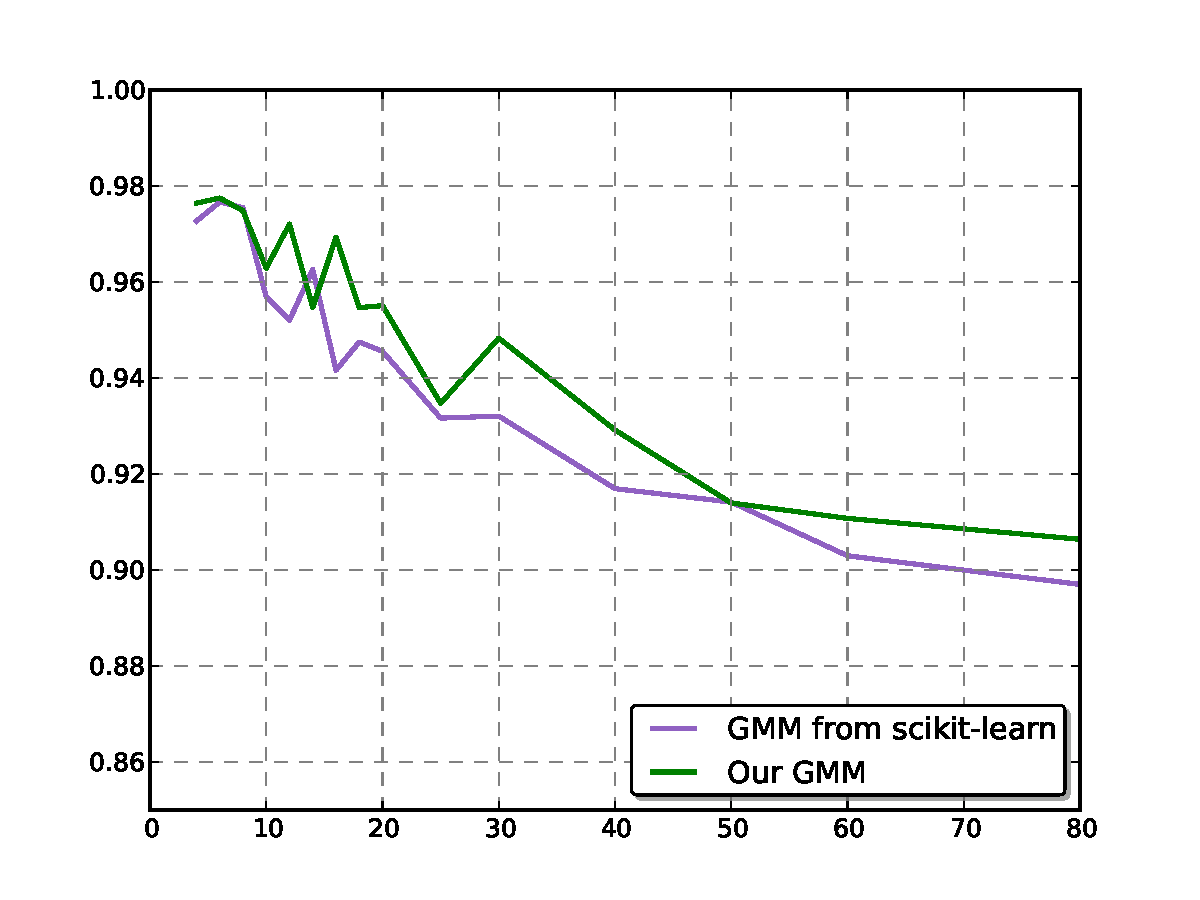
\includegraphics[width=\linewidth]{img/gmm-compare.pdf}
	\caption{Accuracy curve for two GMM}
\end{figure}

From this graph we could see that, our GMM performs better than GMM from scikit-learn in general.
Due to the random selection of test data,
the variance of the test can be high when the number of speakers is small,
as is also the case in the next experiment. But this result still shows that
our optimization on GMM takes effect.

\subsection{Accuracy Curve on Different Number of Speakers}

An apparent trade-off in speaker recognition task is the number of speakers
enrolled and the accuracy on recognization.
Also, the duration of signal for enrollment and test can have significant effect on the accuracy.
We've conducted test using well-tuned parameters for feature extraction as well as GMM, on dataset with
various number of people and with various test duration.

The configurations of this experiment is as followed:
\begin{itemize}
  \item Database: ``Style-Reading''
  \item MFCC: frame size is $32 ms $, 19 cepstrums, 55 filterbanks
  \item LPC: frame size is $32 ms $, 15 coefficients
  \item GMM from scikit-learn, number of mixtures is 32
  \item 20s utterance for enrollment
  \item 50 sampled test utterance for each user
\end{itemize}

\begin{figure}[H]
  \centering
  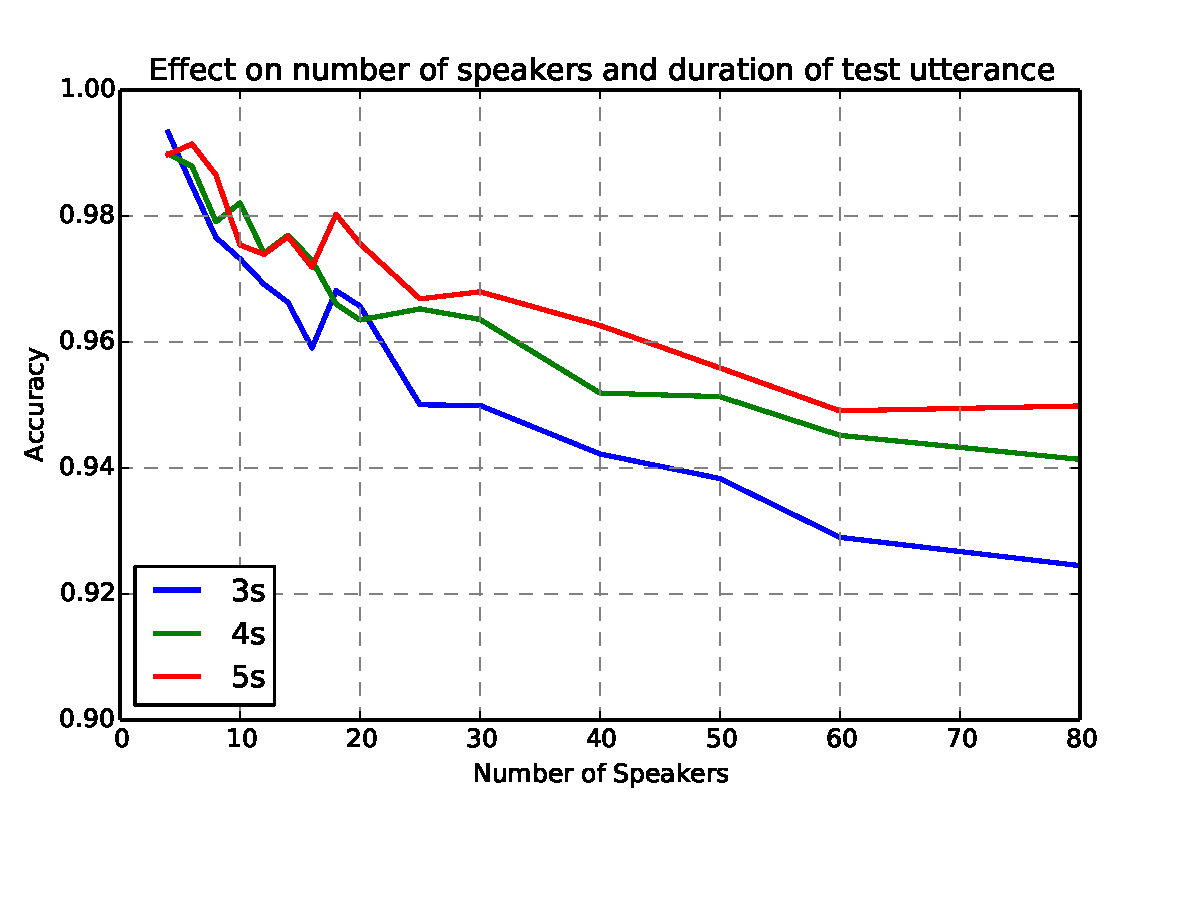
\includegraphics[width=0.9\textwidth]{img/performance.pdf}
\end{figure}

We also conducted experiments on different style of corpus.
The configurations of this experiment is as followed:
\begin{itemize}
  \item MFCC: frame size is $32 ms $, 15 cepstrums, 55 filterbanks
  \item LPC: frame size is $32 ms $, 23 coefficients
  \item GMM from scikit-learn, number of mixtures is 32
  \item 20s utterance for enrollment
  \item 50 sampled test utterance for each user
\end{itemize}

The result is shown below. Note that each point in the graph is an
average value of 20 independent test with random sampled speakers .

\begin{figure}[H]
  \centering
  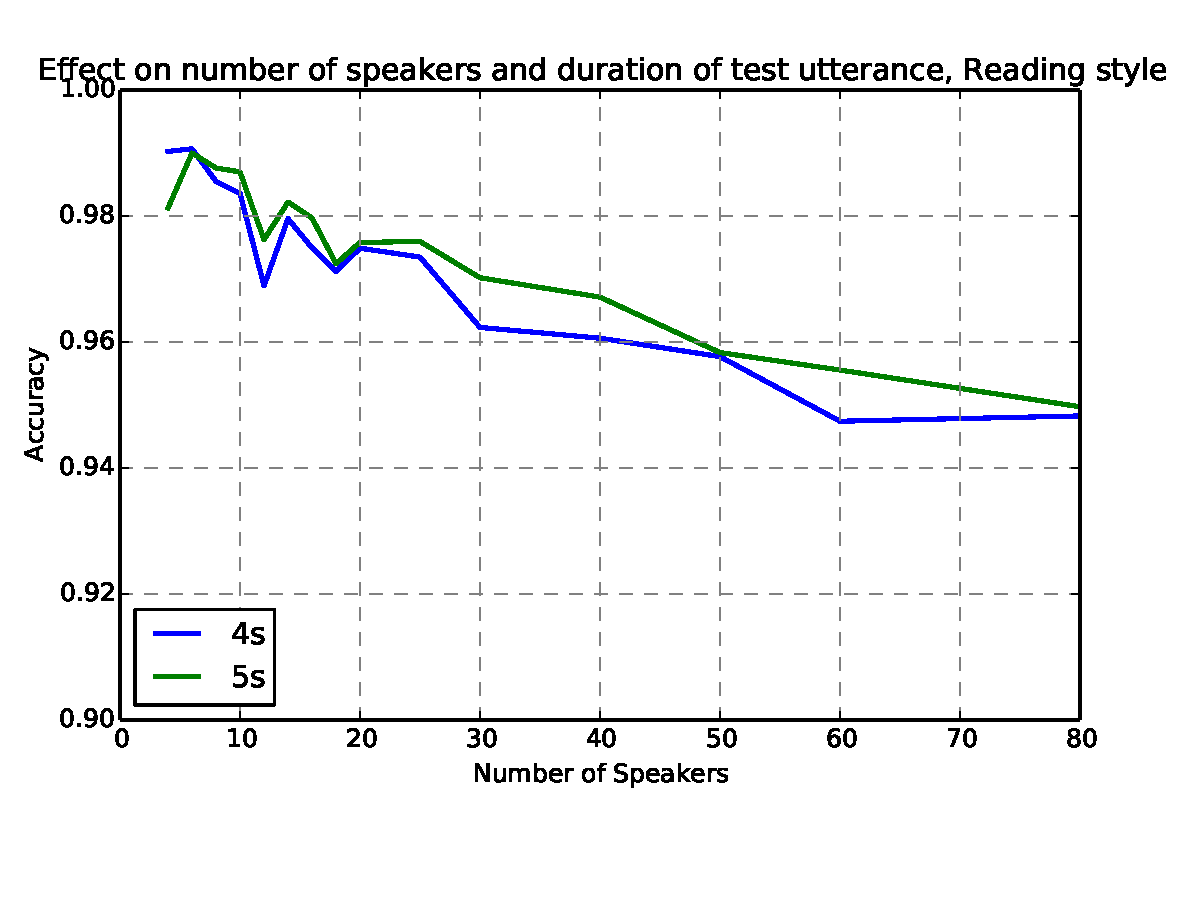
\includegraphics[width=0.9\textwidth]{img/reading.pdf}
\end{figure}
\begin{figure}[H]
  \centering
  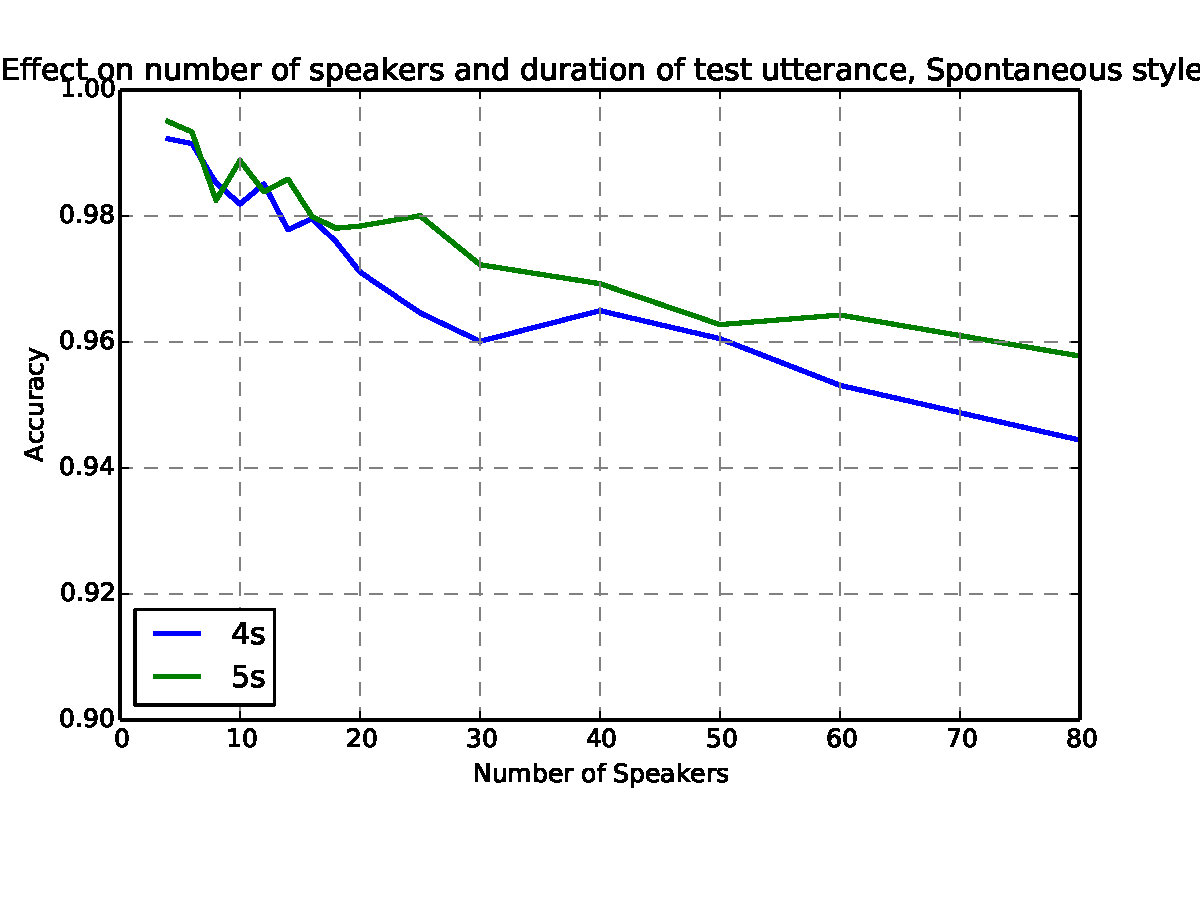
\includegraphics[width=0.9\textwidth]{img/spont.pdf}
\end{figure}

\begin{figure}[H]
  \centering
  \includegraphics[width=0.9\textwidth]{img/whisper.pdf}
\end{figure}

\subsection{CRBM Performance Test}
We also tested RBM using following configuration:
\begin{itemize}
  \item MFCC: frame size is $32 ms $, 15 cepstrums, 55 filterbanks
  \item LPC: frame size is $32 ms $, 23 coefficients
  \item CRBM with 32 hidden units.
  \item 50 sampled test utterance for each user
  \item 5s test utterance
\end{itemize}

\begin{figure}[H]
  \centering
  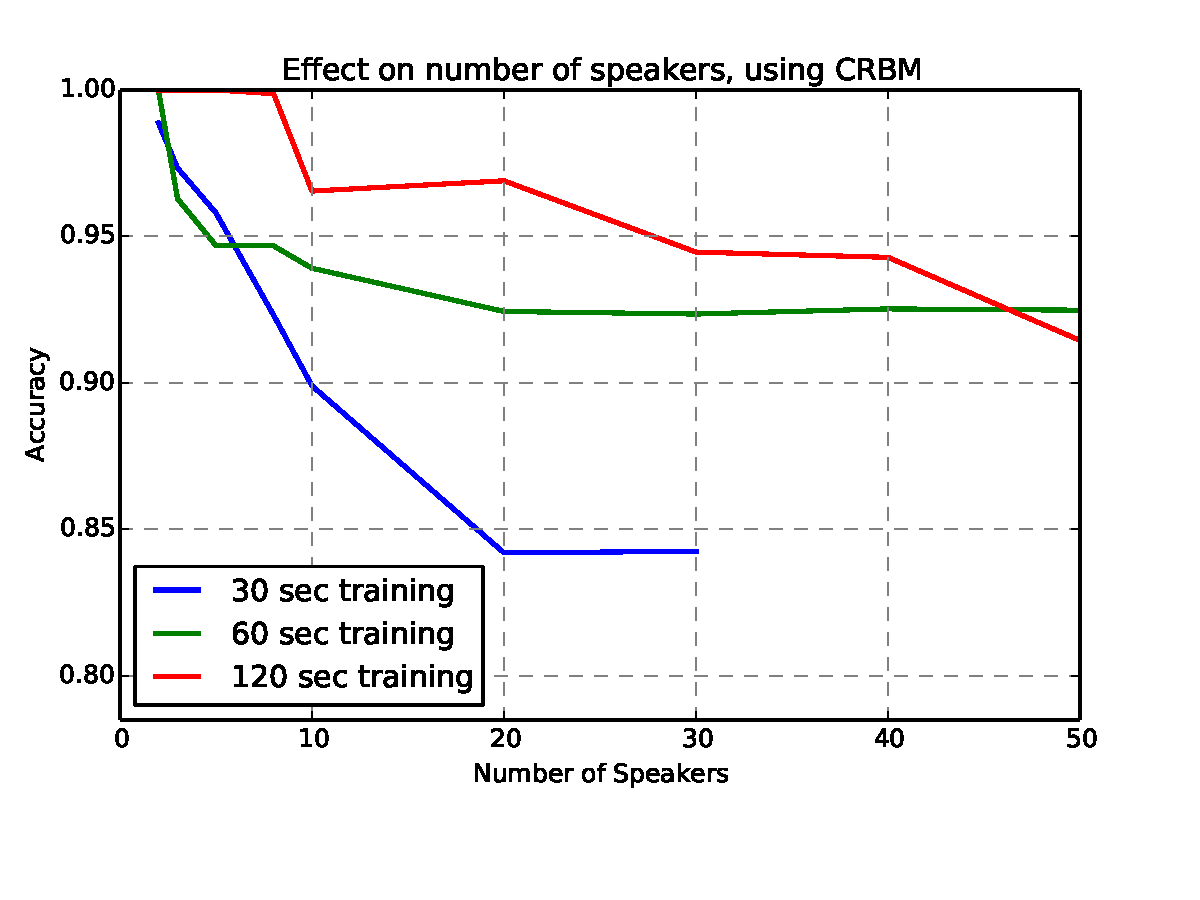
\includegraphics[width=0.9\textwidth]{img/crbm.pdf}
  \caption{\label{fig:crbmresult}}
\end{figure}

Result shown in \figref{crbmresult} indicates that, although CRBM have
generic modeling ability, applying it on signal features does not fit
our expectation. To achieve similar results, the training utterance should
be twice as large as GMM used. Further investigation on using RBM to
process signal features need to be conducted.


